\section{基于数据驱动的基因调控网络构建方法}
\label{sec:d3grn}

\subsection{引言}

从基因表达数据推断基因调控网络~(GRNs)~是系统生物学中一个具有挑战性的基础问题。
在上一章中我们提出了一种基因调控网络的结构推断方法,
Loc-PCA-CMI~输出的是无向网络,基因和基因之间的权重表示的是调控相互作用关系的强弱。
很多时候我们除了关注基因之间的相互作用之外,还对调控的具体方向十分感兴趣。
为了构建有向网络,现有的一些流行的算法将~GRN~推理表述为回归问题,并以聚合~(ensemble)~策略获得最终的网络。
最近关于数据驱动的动态网络构建的研究,主要是偏微分方程和机器学习相结合, 
为我们利用回归方法研究基因调控网络提供了一个全新的视角。
在本文的研究中,我们提出了一种改进数据驱动的动态网络构建方法来推断基因调控网络,命名为~D3GRN。
该方法将每个目标基因的调控关系转化为函数分解问题,利用改进后的揭示网络相互作用的算法~ARNI~解决各个子问题。
为了弥补~ARNI~仅从单元级构建网络的局限性,我们采用抽样~(bootstrapping)~和基于面积的评分方法~(area-based scoring)~来推断最终的网络。
实验结果表明, 在~DREAM4~和~DREAM5~基准数据集上, D3GRN~在~AUPR~这个评价指标上优于最先进的算法。

\subsection{相关工作}

在~DREAM~系列竞赛的推动下,大量研究人员采用机器学习回归模型对基因调控网络进行构建。
这类方法本质上可以看作是关联网络模型的延伸,
不同的是,关联网络只关注量化相互作用,回归方法则能推断出基因之间的相互作用方向。
回归模型将基因调控建模转化为机器学习特征选择的问题,
也就是将目标基因的表达看作是调控基因表达之间的相互线性作用或者非线性作用的结果,
然后结合~bagging~或者~boosting~的思想,推断出最终的基因调控网络。
GENIE3~\cite{huynh2010inferring}~被认为是在一些基准数据集的最好方法~\cite{marbach2010revealing},
该方法是基于随机森林训练了一个回归模型,为每个基因挑选出最重要的调控因子。
在~GENIE3~基础上,~GRNBoost2~\cite{moerman2019grnboost2}~做了扩展, 适合于有成千上万个基因的大规模数据集。
所不同的是,它是通过使用随机梯度增强的机器学习回归方法来进行特征选择, 
并加入正则化和``early stop"~机制来防止模型过拟合。 
TIGRESS~\cite{Haury2012}~使用最小角回归~(LARS)~并结合稳定性选择来解决~GRN~的推断问题。
NIMEFI~\cite{ruyssinck2014nimefi}~研究了合并几种特征选择方法的潜在效果,
例如~GENIE3,~集成支持向量回归~(E-SVR)和~集成弹性网络~(E-EL)~\cite{zou2005regularization},
并在一般框架下结合这些方法对最终的基因调控网络进行预测。
bLARS~\cite{singh2016blars}可以视为~TIGRESS~的变种方法,
其中调控关系是从预定义的基础函数建模取得的,并且通过修改的~LARS~算法推断出最终的~GRN。

最近几年尤其是在物理领域中,数据驱动的动态网络构建是一个非常有吸引力的课题。
SINDy~\cite{brunton2016discovering}~假设只有少数重要变量可以控制动态系统,
因此,偏微分方程在潜在的函数空间中是稀疏的。
然后,它使用稀疏回归来准确确定表示数据所需要的动态控制方程中的少数项。
ARNI~\cite{casadiego2017model}~是一个独立于模型的框架,依赖于它们的非线性聚合动力学, 来推断网络动态系统中的直接交互作用。
它在最终实现的时候是通过函数分解和基函数的展开来求解非线性微分方程组。

虽然~bLARS,~SINDy~和~ARNI~是在不同的研究领域提出来的,
它们的基本思想十分相似。
我们从三个不同的方面对这三个方法进行比较, 如表~\ref{comparision}~所示。
形式化函数分解~(formal function  decomposition)~意味着该方法是否具有函数分解方程的形式描述;
稀疏组约束~(sparse group  constraints )~指示该方法是否利用候选项的稀疏组约束,
而基于网络的构造~(network based construction)~表明该方法是否能重建整个网络结构。
~SINDy~和~ARNI~都没有解决从网络层面发现物理机制的问题,它们仅侧重于某一个特定节点。
由于目前还没有一种方法能覆盖​​这三个方面,
所以在本研究中,我们第一次尝试将上述三个方面合为一体,提出了一种新的数据驱动的动态网络构建方法。
~D3GRN~将每个靶基因的调节关系转化为函数分解问题并以特征选择的方式解决每个子问题,
通过使用~ARNI~算法揭示网络相互作用结构。
使用基于面积的评分方法通过聚合策略推断整个网络结构。
我们在~DREAM4~和~DREAM5~基因调控网络重建竞赛数据集上将方法~D3GRN~与其它几种当今表现最好的基准方法进行比较,
结果表明~D3GRN~在~AUPR~上具有优势。

\begin{table}[!htbp]
    %\caption{Comparison of the related methods}
    \caption{相关方法比较}
    \centering
%    \begin{adjustbox}{max width=0.5\textwidth}
    \label{comparision}  
    \begin{tabular}{lccccc}
    \toprule
    &bLARS &SINDy&ARNI&D3GRN\\
    \midrule
    formal function  decomposition &$\times$ &\checkmark &\checkmark&\checkmark\\ 
    sparse group  constraints &\checkmark &$\times$ &\checkmark&\checkmark\\
    network based construction&\checkmark&$\times$ &$\times$&\checkmark\\
    \bottomrule                   
    \end{tabular}
  %  \end{adjustbox}
\end{table}

\subsection{基于数据驱动的基因调控网络构建方法~D3GRN}
% \subsubsection{问题定义}

如果不考虑基因之间的上游或下游调节关系并且忽略自我调节机制,则可以将~GRN~视为有向无环图~(directed acyclic graph,~DAG)。
在~DAG~中,每个节点对应于基因,并且每个边缘代表基因之间的调节关系。
和许多其它聚合方法一样~(例如~\cite{huynh2010inferring,Haury2012,slawek2013ennet,ruyssinck2014nimefi,guo2016gene,zheng2019ensemble}),
它不利用不同实验条件的信息~(例如,基因敲除,扰动甚至重复),
我们仅基于基因表达数据使用~GRN~推理问题的通用框架。
作为输入基因表达数据,我们考虑在~$M$~实验条件下测量~$N$~基因的表达量。
因此,基因表达数据~$A$~定义如下:
\begin{equation}
\label{eq:definion}
A = [x_1,x_2,\ldots,x_N] \in \mathbb{R} ^ {M \times N}
\end{equation}
其中~$x_i$~是所有~$M$~实验条件中第~$i$~个基因的表达值的列向量。

GRN~推断方法预测基因表达数据基因之间的调节关系~$A$。
大多数方法提供了从最高到较低置信度的潜在调控关系的排序列表。
随后可以通过在该排序列表上使用变化的阈值来获得不同的~DAG。
因为最终用户可以自由探索各个阈值水平的网络~\cite{slawek2013ennet},
本研究中我们只关注列表的排序问题。
值得注意的是,排序是``逆向工程对话评估和方法"~(DREAM)~\cite{stolovitzky2007dialogue}竞赛的标准预测格式,
其中已经提出了各种~GRN~推断方法。
此外,我们不考虑从排序中获得的网络的稳定性。

为了从表达数据~$A$~推断出调控网络,
我们计算一个权重分数~$S_{ij}$,
表示基于基因表达水平值上基因~$i$~调控基因~$j$的强度~(包括上调和下调)。

% \subsubsection{基于集成回归方法的网络推理}

受基于特征选择的集成方法,例如~GENIE3~\cite{huynh2010inferring}~和~TIGRESS~\cite{Haury2012}~成功被应用的启发,
$n$~个基因的~GRN~推断问题可以分解为~$n$~个子问题,
其中每个子问题都可以看作是机器学习中的特征选择问题~\cite{nasrabadi2007pattern}。
更具体地说,对于每个目标基因,我们希望从表达水平上确定直接影响它的基因子集。
设~$A$~是等式~(\ref{eq:definion})~中定义的基因表达数据,
第~$i$~个基因为靶基因,我们在~$M$~个实验条件~(即样本)~下定义了其它候选表达调控因子:
\begin{equation}
  \label{eq:x}
  x^{-i} = [x_1,\ldots,x_{i-1},x_{i+1},\ldots,x_N]
  \end{equation}

特征选择问题可以表示为:
\begin{equation}
\label{eq:fs}
x_i =  F(x^{-i}) + \epsilon , \forall i \in \{1,2,\ldots,N\}
\end{equation}
其中,~$F$~是任意一个平滑, 典型的如~$x^{-i}$~个基因~(也就是跟基因~$i$~相关的基因)~表达值的非线性函数;~$\epsilon$~是噪声项~\cite{huynh2010inferring,Haury2012}。
% Generally, the function $F$ is unknown which can be defined indirectly as:
% \begin{equation}
% \label{eq:ffunction}
% F(x^{-i}) = \sum_{1}^{n} w_{ji}x_j , \forall j \in \{1,\ldots,i-1,i+1,\ldots,n\}
% \end{equation}
% where $w_{ji}\geqslant 0$ represents the strength~(or confidence) that gene $i$ associates (i.e., regulates) gene $j$. 
% The rankings of the regulatory links of gene $i$ is obtained by computing the $w_{ji}$.
把~$N$~个独立的基因排序聚合起来,我们能得到一个全局的~GRN~的调控关系的排序。

% \subsubsection{使用~D3GRN~进行~GRN~推断}

D3GRN~算法的伪代码如算法~\ref{alg:D3GRN}~所示。
其中,~$A_j$~指的是矩阵~$A$的第~$j$~列,~$A_I$~是~$A$~中包含索引列集合~$I$~的子矩阵。

假定,输入的基因表达矩阵~$A \in \mathbb{R}^{M \times N}$, 
并且转录因子的索引~$I \subset \{1,\ldots,N\}$, 
同时抽样数目和~ARNI~算法的步数~$L$~已经知道。
在~$A$~中放回重复抽样,针对第~$i$~次抽样,对于每一个目标基因~$j$, 
对应的目标基因~$j$~的表达值为~$y$, 
其它的转录因子~$X$~的表达值也被获取到。
ARNI~算法调用后,返回的是被选中的调控因子~$SM_j$~的一个有序列表~(ordered list)。
最后,在所有的~$b$~轮抽样结束后,
矩阵~$SM$~作为输入变量,通过基于面积的打分方法,
我们赋予一个候选的转录因子和目标基因之间的边~0~和~1~之间的分数。
抽样和基于面积的打分方法的细节,以及计算复杂度分析,我们在后续的章节中会详细介绍。
 
\begin{algorithm}
  %\caption{D3GRN Pseudo Code}
  \caption{D3GRN~算法伪代码}
  \label{alg:D3GRN}
  \begin{algorithmic}[1]
  \Require  $A \in \mathbb{R}^{M \times N}$, $I \subset \{1,\ldots,N\}$, 
            $|I| = n$,
            $b$(the number of bootstrapping runs), $L$(ARNI steps) %\Comment{Number of bootstrapping runs and ARNI steps}
  \Comment{$M$ samples, $N$ genes, I index set of $n$ regulators}
  
  \Ensure The score matrix $S$ 
  \State Initialize $S \in \mathbb{R}^{N \times n}$     \Comment{Initialize adjacency matrix of the GRN}
  \State Initialize $SM \in \mathbb{R}^{n \times b}$     \Comment{Initialize the selection matrix}
  \For{$i = 1 \to b$}                                   \Comment{For each bootstrapping run}
        \State $A^{*}$ = resample$(A)$                  \Comment{Resampling with replacement}
        \For{$j = 1 \to n$}                             \Comment{For each target gene}         
        \State $y = A^{*}_j, X = A^{*}_{I\setminus j}$
        \State $SM_{ji}$ = ARNI$(y,X,L)$                    \Comment{Returns selected tx-factors with the ARNI algorithm}
        \EndFor
  \EndFor           
  \State $S$ = area-score$(SM,L,b)$                      \Comment{Get the weight score matrix with the area-score metric}
  \State \Return $S$                                    \Comment{Output the score matrix}
\end{algorithmic}
\end{algorithm}

\subsubsection{基于~ARNI~的特征选择}

对于给定节点~$i$~及其对应的微分方程, 
ARNI~转向获得哪些节点~$j$~的网络提供了直接的物理相互作用, 并出现在等式的右侧, 
而不是探索方程中这些节点之间的交互函数的细节。

详细地, 对于~$N$~个节点的动态系统, 
ARNI~首先将单元~$i$~的动态性分解为与网络中其它单元的交互项~\cite{casadiego2017model}:
\begin{equation}
\label{eq:xi}
\begin{split}
% \dot{x_i}= & f_i(\Lambda ^i x)\\
%          = &\sum_{j=1}^{N} \Lambda^i_{jj} g^i_j(x_j) + 
%                              \sum_{j=1}^{N} \sum_{s=1}^{N}\Lambda^i_{jj}\Lambda^i_{ss}g^i_{js}(x_j,x_s)\\
%          + &\sum_{j=1}^{N} \sum_{s=1}^{N} \sum_{w=1}^{N}\Lambda^i_{jj}\Lambda^i_{ss}\Lambda^i_{ww}g^i_{jsw}(x_j,x_s,x_w)+ \ldots + \epsilon_{i}
% \end{split}
\dot{x_i}= & f_i(\Lambda ^i x)\\
         = &\sum_{j=1}^{N} \Lambda^i_{j} g^i_j(x_j) + 
                             \sum_{j=1}^{N} \sum_{s=1}^{N}\Lambda^i_{j}\Lambda^i_{s}g^i_{js}(x_j,x_s)\\
         + &\sum_{j=1}^{N} \sum_{s=1}^{N} \sum_{w=1}^{N}\Lambda^i_{j}\Lambda^i_{s}\Lambda^i_{w}g^i_{jsw}(x_j,x_s,x_w)+ \ldots + \epsilon_{i}
\end{split}
\end{equation}

其中~$\dot{x}_i :=[\dot{x}_{i,1}, \dot{x}_{i,2},\ldots,\dot{x}_{i,M}]\in \mathbb{R}^M$,
$f:\mathbb{R}^N \to \mathbb{R}$~是一个平滑函数, 
对角矩阵~$\Lambda^i \in \{0,1\}^{N \times N}$~中~$\Lambda^i_{j}=1$~如果~$j$~直接作用于~$i$, 
否则~$\Lambda^i_{j}=0$,~$g^i_j:\mathbb{R} \to \mathbb{R}$, $g^i_{js}:\mathbb{R}^2 \to \mathbb{R}$, $g^i_{jsw}:\mathbb{R}^3 \to \mathbb{R}$,
并且一般~$g^i_{j_{1}j_{2}\ldots\\j_{K}}:\mathbb{R}^K \to \mathbb{R}$~表示(未知)单元~$j_k$~($k \in \{1,2,\ldots,K\}$)~和单元~$i$~的第~$K$~阶相互作用, 
最后一项~$\epsilon_{i}$~代表于作用于~$i$~的额外噪声。

函数~$g^i_{j_{1}j_{2}\ldots\\j_{K}}$~无法访问~\cite{casadiego2017model},可以将其分解为基函数~$h$,
我们可以将等式~(\ref{eq:xi})~重写为:
\begin{equation}
\label{eq:xi_with_h}
\begin{split}
% \dot{x_i} =  &\sum_{j=1}^{N} \Lambda^i_{jj} \sum_{p=1}^{P_1} c^i_{j,p}h_{j,p}(x_j) \\
% + &  \sum_{j=1}^{N} \sum_{s=1}^{N}\Lambda^i_{jj}\Lambda^i_{ss} \sum_{p=1}^{P_2} c^i_{js,p}h_{js,p}(x_j,x_s) \\
%                              + &\sum_{j=1}^{N} \sum_{s=1}^{N} \sum_{w=1}^{N}\Lambda^i_{jj}\Lambda^i_{ss}\Lambda^i_{ww} \sum_{p=1}^{P_3} c^i_{jsw,p}h_{jsw,p}(x_j,x_s,x_w)\\
%                              + &\ldots + \epsilon_{i} 
% \end{split}
\dot{x_i} =  &\sum_{j=1}^{N} \Lambda^i_{j} \sum_{p=1}^{P_1} c^i_{j,p}h_{j,p}(x_j) \\
+ &  \sum_{j=1}^{N} \sum_{s=1}^{N}\Lambda^i_{j}\Lambda^i_{s} \sum_{p=1}^{P_2} c^i_{js,p}h_{js,p}(x_j,x_s) \\
                             + &\sum_{j=1}^{N} \sum_{s=1}^{N} \sum_{w=1}^{N}\Lambda^i_{j}\Lambda^i_{s}\Lambda^i_{w} \sum_{p=1}^{P_3} c^i_{jsw,p}h_{jsw,p}(x_j,x_s,x_w)\\
                             + &\ldots + \epsilon_{i} 
\end{split}
\end{equation}
其中,~$P_k$~表示扩展函数中采用的基函数数目~\cite{friedman2001elements}。
$c^i_{j,p}$,~$c^i_{js,p}$,~$c^i_{jsw,p}$~为未知系数。
适当的基函数~$h$~有利于形成相关的函数空间。
例如,对偶基函数类~$g^i_{ij}(x_i,x_j)$~可以是~$h^i_{ij,p}(x_i,x_j)=(x_j-x_i)^p$~或~$h^i_{ij,p}(x_i,x_j)=x^{p_{1}}_i x^{p_{2}}_j$~等形式。

需要注意的是, 该框架旨在揭示动态系统中各单位的直接交互作用,尤其是时间序列数据。
对于~GRN~推理问题,尤其是来自非时间序列数据的推理,
可以对等式~(\ref{eq:xi_with_h})~做一个修改。
更特别的是,将等式~(\ref{eq:xi_with_h})~中左边的时变项~$\dot{x_i}$~替换为一个非时间变化的项~$x_i$, 注意这是一个矢量。
不考虑自我作用的同时,修改后的方程可以定义为:
\begin{equation}
\label{eq:x_i_fs}
% \begin{split}
% x_i = &\sum_{j=1}^{N} \Lambda^i_{jj} \sum_{p=1}^{P_1} c^i_{j,p}h_{j,p}(x_j)\\  
%     + &\sum_{j=1}^{N} \sum_{s=1}^{N} \sum_{w=1}^{N}\Lambda^i_{jj}\Lambda^i_{ss}\Lambda^i_{ww} \sum_{p=1}^{P_3} c^i_{jsw,p}h_{jsw,p}(x_j,x_s,x_w)\\
%     +&\ldots + \epsilon_{i}, \forall jj,ss,ww \in \{1,\ldots,i-1,i+1,\ldots,N\}
% \end{split}
\begin{split}
   x_i = &\sum_{j=1}^{N} \Lambda^i_{j} \sum_{p=1}^{P_1} c^i_{j,p}h_{j,p}(x_j)\\  
       + &\sum_{j=1}^{N} \sum_{s=1}^{N} \sum_{w=1}^{N}\Lambda^i_{j}\Lambda^i_{s}\Lambda^i_{w} \sum_{p=1}^{P_3} c^i_{jsw,p}h_{jsw,p}(x_j,x_s,x_w)\\
       +&\ldots + \epsilon_{i}
   \end{split}
\end{equation}

从等式~(\ref{eq:xi_with_h})~到等式~(\ref{eq:x_i_fs})~的转换很自然。
在这种情况下,等式~(\ref{eq:x_i_fs})~就是等式~(\ref{eq:fs})~的详细实现。
重构问题就变成了识别等式~(\ref{eq:x_i_fs})~中的非零相互作用项。
系数向量~$c^i_{j,p}$,~$c^i_{js,p}$,~$c^i_{jsw,p}$~是未知的,
阻碍了~$\Lambda^i$~的计算。
在等式~(\ref{eq:x_i_fs})~中加上一个由零和非零系数组成的块状结构约束即可,
分别代表不存在和现有的相互作用。
这些结构化的解是由沿~$c^i$~分布的非零条目~(代表作用于单位~$i$~的非零交互作用)的块~$c^i_s$~构成的。
提出了揭示网络交互作用的算法~ARNI~来解决这个数学分组变量的回归问题。
这是一种基于块正交最小二乘~(BOLS)~算法的贪心方法~(greedy method)~\cite{majumdar2009fast}。
ARNI~在本质上可以看作是一种合适的特征选择方法,
与知名的~Sparse Group Lasso~\cite{friedman2010note}~有类似之处。
该算法的细节在文献~\cite{casadiego2017model}~的补充文档中有很详细的陈述。

\subsubsection{抽样方法}

D3GRN~算法采用抽样方法,以获得更可靠的目标基因的调控因子选择。
一般来说,抽样~\cite{efron1994introduction}~是用于从经验分布的中估计参数。
抽样~\cite{efron1994introduction}~从经验分布中产生多组样本。
通过从观察样本中重采样, 然后计算每个重采样集里面的未知参数。
最后, 通过对所有重新采样的集合进行平均,就可以得到有关参数的估计值。
在重采样中, 从观察样本中均匀随机,有替换地抽取样本。
重采样技术经常被应用于在欠确定问题的情况下得到稳定的结果~\cite{wang2011random}。
在当前的~D3GRN~实现中,抽样次数~$b$=200。
在每次抽样过程中, 
~$y$~和~$X$~是从给定的基因表达数据中均匀随机选择重新采样与替换。
随后,~ARNI~算法被用来选择每次抽样后与目的基因有关的调控因子。
最后,所有抽样的结果使用基于面积的评分~\cite{Haury2012}~技术进行汇总。
需要注意的是,~D3GRN~算法只应用抽样方法来获得每个目标基因的高置信度调控因子,
并不是同~\cite{Haury2012}~那样在许多抽样网络上进行汇总。

\subsubsection{基于面积的评分}
基于面积的评分法~(area-based scoring})~是根据它在指定的抽样中的频率,
给每个候选调控因子进行打分。
在每次抽样中, 
~ARNI~提供的目标基因的调控因子的有序列表在数学上是独立的。
这种评分方法需要利用被选择到的调控因子的整体排序信息。
我们使用通过基于面积的评分方法来实现这个目的。

设~$\phi_{ijl}$~为第~$j$~个调控因子在~ARNI~的第~$l$~步中的累积选择频率。
$l={1,\ldots,L}$,显然~$\phi_{ijl}$~在~$[0,1]$。
平均值取所有抽样的平均值, 
基因~$i$~的调控因子~$j$~在总~$L$~步数中的得分~$S_{ij}$~定义为:
\begin{equation}
\label{eq:scoring}
S_{ij} = \frac{1}{L} \sum_{l=1}^{L} \phi_{ijl}
\end{equation}

例如,假定~$\phi_{ij1}=0.3$,~$\phi_{ij2}=0.5$,~$L=5$。
在第~5~个步骤中,第~$j$~个调控因子在第一个~ARNI~步骤中~30\%~的次数被选择,
在第二个~ARNI~步骤中~20\%~的次数被选择,那么累计选择频率~$\phi_{ij2}$~为~50\%。
分数~$S_{ij}$~有一个自然的解释,即由总面积~L~归一化的累积选择频率曲线下的面积。
%在~GRN中,得分~$s_j$代表调节器~$j$和目标基因~$i$的调控边的大小~$w_{ji}$,这在等式~(\ref{eq:function})中有所描述。
显然,这个分数不仅考虑了转录因子的总体选择频率,而且还倾向于奖励在每个~ARNI~步骤中较早被选择出来的调控因子。
与基于整体选择频率~$\phi_{ij}$~的简单排序相比,这种方法对~ARNI~步骤的敏感性较低。

\subsubsection{计算复杂度}

算法的计算复杂度主要取决于~ARNI,针对于每个目标基因复杂度为~$O(t^2*(tp)^3)$。
其中~$t$~为转录因子的数目,~$p$~为基本函数的数目~(即方程~(\ref{eq:xi_with_h})中的~$P_k$)。
$O((tp)^3)$~是由于~BOLS~算法的~Moore-Penrose~伪逆复杂性。
因此,该算法的总体计算复杂度为~$O(t^5p^3nb)$。
其中,~$n$~是目标基因的数量,~$b$~是抽样数,由于~$t$~通常比~$n$~小得多,时间复杂度的上界是~$O(n^6p^3b)$。
由于~$t$~通常比~$n$~小得多, 所以时间复杂度的上界是~$O(n^6p^3b)$。
算法~\ref{alg:D3GRN}~中的``for"循环是完全可以并行的,可以在多核甚至分布式集群机器上同时进行。


\subsection{实验结果}

\subsubsection{数据集}

在过去十年中,~GRN~推理一直是一个相当活跃的研究领域。
因此,一个名为``逆向工程对话"的社区联合体~(DREAM)\cite{stolovitzky2007dialogue}成立,
在过去十年中一直在积极地研究~GRNs~推理。
DREAM~联盟举办国际逆向工程挑战赛, 提供标准化的通用输入数据集和性能评估指标来比较不同的方法。
该组织提供的数据集成为了~GRN~推理领域的金标准, 经常用于评估新算法的性能。

在实验中,
我们使用~DREAM4~和~DREAM5~挑战赛中的~6~个模拟数据集~\cite{marbach2012wisdom}。
数据集详情如表~\ref{datasets}~所示,其中~Network~表示数据集名称,
\#Genes~表示基因的数量, \#Regulators~表示调控因子的数量, \#Samples~表示样本的数量, 
\#Verified interactions~表示网络中的有向调控边数。
如果一个数据集用矩阵表示,那么行表示样本,列表示基因。
我们采用~DREAM4~挑战赛中的~5~个多因素数据集,
每个包含~100~个基因和~100~个样本。
这~5~个数据集中的样本是通过从原始数据中同时微扰动所有基因表达值, 借助于使用开源的~GeneNetWeaver~软件~\cite{marbach2009generating}生成的。
因此,这~5~个数据集中的每个样本都代表了一个多因素扰动实验。
调控因子可以被看作是这些基因本身,因为在这几个小网络中竞赛方并没有指定哪些基因是调控因子。
%此外,我们从~DREAM5~数据集中选用了三个不同的和大小变化的网络。
我们还采用了一个~DREAM5~数据集~1,这也是一个由~GeneNetWeaver~模拟生成的网络。
这个模拟网络的拓扑结构是基于模型生物的已知~GRNs。
与~DREAM4~中的网络不同的是,
DREAM5~数据集中的转录因子~(TFs)~是作为调控因子显式提供的,它是提供的所有基因中一个子集。

% while the other two expression datasets are real expression data collected 
% for E. coli (Network 3) and S. cerevisiae (Network 4). 
% It is observed that the performance of previous studies imply that Network 3 and Network 4 
% tend to be almost in a random manner.
% Accordingly, we only employ Network 1 dataset from DREAM5 datasets.
%as Network 3 and Network 4 in DREAM5 are more sparser than Network 1,
% Network 2 of DREAM5 is neglected in our experiments, 
% because there are no verified interactions provided for this dataset. 
% Network 3 and Network 4 in DREAM5 are more sparser than Network 1, 
% as they own more genes and regulators but less interactions.

\begin{table}[!htbp]
\centering
%\caption{Detail of the datasets}
\caption{实验数据集详情}

\label{datasets}
\resizebox{\columnwidth}{!}{%
\begin{tabular}{lccccc}
\toprule
Network           & \#Genes & \#Regulators & \#Samples & \#Verified interactions \\
\midrule
DREAM4  Network 1  & 100     & 100                & 100       & 176                      \\
DREAM4  Network 2  & 100     & 100                & 100       & 249                      \\
DREAM4  Network 3  & 100     & 100                & 100       & 195                      \\
DREAM4  Network 4  & 100     & 100                & 100       & 211                      \\
DREAM4  Network 5  & 100     & 100                & 100       & 193                      \\
%\hline
DREAM5 Network 1   & 1643    & 195                & 805       & 4012                   \\
%DREAM5 Network 3~(E. coli)       & 4511    & 334                & 805       & 2066                     \\
%DREAM5 Network 4~(S. cerevisiae) & 5950    & 333                & 536       & 3940                     \\
\bottomrule                   
\end{tabular}
}
\end{table}

\subsubsection{评价指标}

为了评估~GRN~推理算法的效果,我们使用准确率-召回率曲线下的面积~(AUPR)~作为评价指标。
除了~AUPR~之外,接收者操作特征曲线下的面积~(AUROC)~也被广泛用于评估效果。
一般来说,~AUROC~和~AUPR~值越高,说明~GRN~预测越准确。
需要注意的是,在稀疏的生物网络中,不存在的边数目~(阴性边)大大超过现有边的数量~(阳性边),
因而~AUPR~比~AUROC~\cite{saito2015precision}~更有参考价值。

我们首先通过比较金标准网络中的调节边和~D3GRN~的排序列表输出前~$q$~条边,
计算出真阳性~(TP)、真阴性~(TN)、假阳性~(FP)~和假阴性~(FN)~边的数量。

%The ROC curve is constructed by plotting the true positive rates~(TPR = TP/(TP + FN)) versus the false positive rates~(FPR = FP/(FP + TN)) for increasing $q$~($q = 1,2,\ldots,m^2$).
精确度-召回曲线是通过绘制精确度~$\frac{\text{TP}}{\text{TP + FP}}$~与召回度~$\frac{\text{TP}}{\text{TP + FN}}$~在增加~$q$~的情况下构建的。
~$q = 1,2,\ldots,N\times(N-1)$,其中~$N$~为基因数。
通过计算曲线下的面积得到~AUPR。
%Similarly, the precision~(TP/(TP + FP)) and recall~(TP/(TP + FN)) curve is plotted for increasing $q$.


\subsubsection{实验结果分析}
%\subsubsection{D3GRN~的实验结果}

等式~(\ref{eq:xi_with_h})~中基函数的类型、阶数~$K$~和基函数的数量~$P_k$~在~ARNI~中的模型分解中起着至关重要的作用。
对于一大类动态系统,使用多项式非线性是充分的~\cite{mangan2016inferring}。
作为参考,在我们基因调控网络的构建中,也采用了多项式基函数,
形式为~$h_{j,p}(x_j)=x_j^p$,基函数的数目表示为: 
\begin{equation}
P_k=\left\{\begin{matrix}
5,  k=1\\ 
0,  k>1
\end{matrix}\right. 
\end{equation}
这隐含表达了我们不考虑一个目标基因的~2~阶及以上的阶的交互作用。
事实上,~bLARS~\cite{singh2016blars}~只考虑了一阶交互作用。
我们在本研究中也遵循这种简化的方式。
换句话说,其它基因对目标基因的调控是基于多项式非线性函数的混合。

D3GRN~中有两个参数,
包括抽样的次数~$b$~和~ARNI~步数~$L$。
图~\ref{fig:performance_dr5}~展示了通过改变~DREAM5~网络~1~的~ARNI~步数和抽样次数这两个参数的结果。
一般来说,较大的抽样次数~$b$~运行时间越长,但是它的性能会越趋于稳定和优异。
然而,D3GRN~的性能对抽样次数相当稳定,只要它大于某一阈值,通常是~200~次左右。
对于~ARNI~的步数~$L$,一个直觉是如果~$L$~接近网络中先验的平均调控因子的数量,
那么结果将是最佳的,可以用~$\frac{2  \times \#\text{Verified interactions}}{\#\text{Genes}}$~估计到。
 
\begin{figure}[!htbp]
\centering
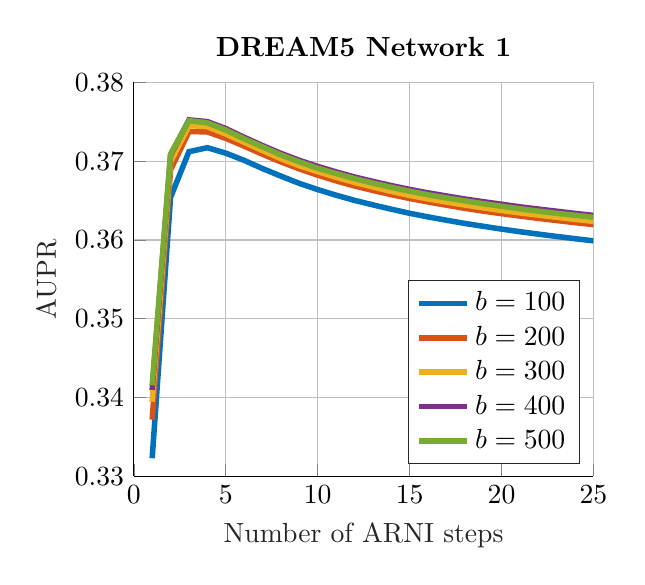
\begin{tikzpicture}

\definecolor{mycolor1}{rgb}{0.00000,0.44700,0.74100}%
\definecolor{mycolor2}{rgb}{0.85000,0.32500,0.09800}%
\definecolor{mycolor3}{rgb}{0.92900,0.69400,0.12500}%
\definecolor{mycolor4}{rgb}{0.49400,0.18400,0.55600}%
\definecolor{mycolor5}{rgb}{0.46600,0.67400,0.18800}%

\newlength{\fheight}
\newlength{\fwidth}
\setlength{\fheight}{5cm}
\setlength{\fwidth}{6cm}

\begin{axis}[%
width=0.973\fwidth,
height=\fheight,
at={(0\fwidth,0\fheight)},
scale only axis,
xmin=0,
xmax=25,
xlabel style={font=\color{white!15!black}},
xlabel={Number of ARNI steps},
ymin=0.33,
ymax=0.38,
ylabel style={font=\color{white!15!black}},
ylabel={AUPR},
axis background/.style={fill=white},
title style={font=\bfseries},
title={DREAM5 Network 1},
axis x line*=bottom,
axis y line*=left,
xmajorgrids,
ymajorgrids,
legend style={at={(0.97,0.03)}, anchor=south east, legend cell align=left, align=left, draw=white!15!black}
]
\addplot [color=mycolor1, line width=2.0pt]
  table[row sep=crcr]{%
1	0.33228\\
2	0.36542\\
3	0.37121\\
4	0.37172\\
5	0.37103\\
6	0.37011\\
7	0.36907\\
8	0.36811\\
9	0.36719\\
10	0.3664\\
11	0.36569\\
12	0.36503\\
13	0.36446\\
14	0.36391\\
15	0.36339\\
16	0.36293\\
17	0.36251\\
18	0.3621\\
19	0.36174\\
20	0.36138\\
21	0.36105\\
22	0.36074\\
23	0.36045\\
24	0.36016\\
25	0.35989\\
};
\addlegendentry{$b=100$}

\addplot [color=mycolor2, line width=2.0pt]
  table[row sep=crcr]{%
1	0.33718\\
2	0.36889\\
3	0.37378\\
4	0.37372\\
5	0.37291\\
6	0.37192\\
7	0.37089\\
8	0.36992\\
9	0.36903\\
10	0.36823\\
11	0.36751\\
12	0.36686\\
13	0.36629\\
14	0.36576\\
15	0.36527\\
16	0.36483\\
17	0.36442\\
18	0.36402\\
19	0.36367\\
20	0.36334\\
21	0.36304\\
22	0.36274\\
23	0.36247\\
24	0.3622\\
25	0.36195\\
};
\addlegendentry{$b=200$}

\addplot [color=mycolor3, line width=2.0pt]
  table[row sep=crcr]{%
1	0.33946\\
2	0.36992\\
3	0.37452\\
4	0.37439\\
5	0.37346\\
6	0.37241\\
7	0.37136\\
8	0.37033\\
9	0.36943\\
10	0.36868\\
11	0.36796\\
12	0.36731\\
13	0.36674\\
14	0.36617\\
15	0.36566\\
16	0.36522\\
17	0.36482\\
18	0.36444\\
19	0.36408\\
20	0.36374\\
21	0.36344\\
22	0.36316\\
23	0.36288\\
24	0.36262\\
25	0.36237\\
};
\addlegendentry{$b=300$}

\addplot [color=mycolor4, line width=2.0pt]
  table[row sep=crcr]{%
1	0.34095\\
2	0.37077\\
3	0.37525\\
4	0.37503\\
5	0.37415\\
6	0.37304\\
7	0.37199\\
8	0.371\\
9	0.37012\\
10	0.36934\\
11	0.36865\\
12	0.368\\
13	0.36744\\
14	0.36691\\
15	0.36642\\
16	0.36598\\
17	0.36559\\
18	0.3652\\
19	0.36486\\
20	0.36454\\
21	0.36421\\
22	0.36392\\
23	0.36365\\
24	0.36337\\
25	0.36312\\
};
\addlegendentry{$b=400$}

\addplot [color=mycolor5, line width=2.0pt]
  table[row sep=crcr]{%
1	0.34154\\
2	0.37091\\
3	0.37515\\
4	0.37487\\
5	0.37396\\
6	0.37285\\
7	0.37182\\
8	0.3708\\
9	0.36992\\
10	0.36911\\
11	0.36844\\
12	0.3678\\
13	0.36722\\
14	0.36669\\
15	0.36619\\
16	0.36574\\
17	0.36534\\
18	0.36497\\
19	0.36461\\
20	0.36428\\
21	0.36396\\
22	0.36366\\
23	0.36338\\
24	0.36314\\
25	0.36288\\
};
\addlegendentry{$b=500$}

\end{axis}
\end{tikzpicture}

%\caption{AUPR by varying ARNI steps $L$ and the bootstrapping number $b$ in DREAM5  Network 1.}
\caption{
在~DREAM5~网络1~上不同的~ARNI~步骤数~$L$~和抽样数目~$b$~取得的~AUPR~值}

\label{fig:performance_dr5}
\end{figure}

我们在~DREAM4~和~DREAM5~网络进行了两次对比实验,来评测我们提出的方法~D3GRN。
NIMEFI~用~R~实现,而~GENIE3、TIGRESS~是用~MATLAB~实现。
这些方法的代码从对应论文提供的~URL~进行下载,在实验中各方法中的参数使用它们代码注释中提供的默认值。
我们提出的方法~D3GRN~也是在~MATLAB~中实现的,使用的数据集及代码公开在~GitHub~仓库~\url{https://github.com/chenxofhit/D3GRN}~上。

表~\ref{tab:performance_dr4}~列出了~D3GRN~与其它~GRN~推理方法在五个~DREAM4~网络上比较的结果。
其中,~D3GRN~的参数是在抽样数~$b=200$,~ARNI~步数~$L=2$~下得到的。
如表所示,除了在~DREAM4网络~2~上,~D3GRN~跟其它方法相比~AUPR~值最高。

表~\ref{tab:performance_dr5}~总结了~D3GRN~与其它~GRN~推理方法在~DREAM5~数据集上的比较结果。
D3GRN~的参数设置为抽样数~$b=200$,ARNI步数~$L=5$。
D3GRN~在网络~1~上跟其它方法相比~AUPR~值最高。

% \begin{table*}[!htbp]
%   %\resizebox{\columnwidth}{!}{%
%   \centering
%   \begin{threeparttable}  
%   \caption{Performance comparisons of different GRN inference methods on the DREAM4 networks, challenge size 100 Multifactorial}  
%   \label{tab:performance_dr4} 
%     \begin{tabular}{ccccccccccc}  
%     \toprule  
%     \multirow{2}{*}{Method}&  
%     \multicolumn{2}{c}{Network 1}&\multicolumn{2}{c}{Network 2}&\multicolumn{2}{c}{Network 3}&\multicolumn{2}{c}{Network 4}&\multicolumn{2}{c}{Network 5}\\
%     \cmidrule(lr){2-3} \cmidrule(lr){4-5}  \cmidrule(lr){6-7}  \cmidrule(lr){8-9} \cmidrule(lr){10-11}
%     &AUPR&AUROC &AUPR&AUROC &AUPR&AUROC &AUPR&AUROC &AUPR&AUROC\\
%     \midrule  
%     GENIE3  &0.161 &0.750        &0.154&0.734         &0.234&0.776          &0.211&0.800         &0.200&0.795    \\
%     TIGRESS &0.158 &0.747        &0.161&0.703         &0.233&0.761          &0.225&0.774         &0.233&0.754     \\
%     NIMEFI  &0.157 &\textbf{0.758}        &0.157&0.731         &0.248&0.776          &0.225&0.806         &0.241&\textbf{0.801}     \\
%     PLSNET  &0.118 &0.713        &\textbf{0.290}&\textbf{0.828}         &0.202&\textbf{0.794}          &0.228&\textbf{0.819}         &0.206&0.786     \\
%     \textbf{D3GRN}    &\textbf{0.175} &0.704        &0.136&0.683         &\textbf{0.253}&0.734          &\textbf{0.255}&0.778         &\textbf{0.247}&0.732     \\
%     \bottomrule  
%     \end{tabular}  
%    \end{threeparttable}
%  %   }
% \end{table*} 

\begin{table}[!htbp]
  %\resizebox{\width}{0.8}{%
  %\resizebox{\textwidth}{20mm}{
  \centering
  \begin{threeparttable}  
%  \caption{Performance comparisons of different GRN inference methods on the DREAM4 networks in terms of AUPR}
  \caption{不同~GRN~推理方法在~DREAM4~网络上的~AUPR~结果}

  \label{tab:performance_dr4} 
    \begin{tabular}{cccccc}  
    \toprule  
    Method
     & Network 1&  Network 2&  Network 3&  Network 4 & Network 5\\
    \midrule  
    GENIE3  &0.161   &0.154           &0.234      &0.211          &0.200                 \\
    TIGRESS &0.158   &\textbf{0.161}           &0.233      &0.225          &0.233                \\
    NIMEFI  &0.157   &0.157           &0.248      &0.225          &0.241                \\
    % PLSNET  &0.118   &\textbf{0.290}  &0.202      &0.228          &0.206                \\
    \textbf{D3GRN}   &\textbf{0.175}  &0.136      &\textbf{0.253} &\textbf{0.255}       &\textbf{0.247}  \\
    \bottomrule  
    \end{tabular}  
   \end{threeparttable}
  %}
\end{table} 

\begin{table}[!htbp]
% \scalebox{0.6}{
% \begin{minipage}{2\linewidth}  
  \centering  
  %\fontsize{6.5}{8}\selectfont  
   % \resizebox{\columnwidth}{!}{%
  \begin{threeparttable}  
%  \caption{Performance comparisons of different GRN inference methods on the DREAM5 Network 1 in terms of AUPR}  
  \caption{不同~GRN~推理方法在~DREAM5~网络~1~上的~AUPR~结果}

  \label{tab:performance_dr5} 
    \begin{tabular}{ccccccc}  
    \toprule  
    Network&GENIE3 &TIGRESS &NIMEFI  &\textbf{D3GRN}\\
    \midrule  
    Network 1&0.291 &0.302 &0.298 &\textbf{0.373}\\
    \bottomrule  
    \end{tabular}  
    \end{threeparttable}
    %}
\end{table} 


\subsection{小结}

在~GRN~推理中, 假设相互作用是稀疏的结构是合理的,
特别是在``小~$n$~大~$p$"的情况下, 即可用样本数量少,基因数量多。
稀疏性约束在机器学习中被广泛应用。
在~GRN~中,稀疏性假设意味着每个基因只有少量的调控因子,这个假设也很合理,
本章提出的~D3GRN~方法也遵循同样的假设。
我们在~DREAM4~和~DREAM5~数据集上评估了我们的方法。
我们认为,其它基因对目标基因的调控是基多项式非线性函数的混合作用。
我们方法的实验结果也验证了这一假设,至于这个假设的理论和生物实验分析需要后续的工作来支持。

另一个重要问题是关于~D3GRN~的计算复杂度。
客观地讲,~ARNI~适合于构建单元级的小型物理动态网络。
ARNI~采用的~BOLS~算法的~Moore-Penrose~伪逆运算,对于大型生物网络来说是很耗时的。
D3GRN~中采用的抽样策略使其在处理大规模~GRNs~推理时更加糟糕。
关于~ARNI~的改进空间,~D3GRN~中抽样策略中的``for"~循环是完全可以并行的,
可以在多核甚至集群中的分布式机器上同时进行。
这也值得其它方法尝试,比如用~BOMP~\cite{majumdar2009fast}来替代~BOLS~算法,这是留给未来的工作。
目前最先进的算法性能的差异性表明,
没有一种算法在所有数据集上都表现得同样出色。
然而,所有这些算法都可以应用于为元算法~(meta algorithm)提供输入,
利用``群体智慧"~(Wisdom of crowds)~来创建一个共识和可靠的社区网络~\cite{Marbach2012a,zheng2008gene}。
另外,从小网络到大网络,所有算法的性能都在下降,这或许反应了不同规模的底层调控网络的复杂性在增加。
我们的方法推进了当前的技术水平, 但要把这个问题完全解决好, 还有很长的路要走。

从基因表达数据中构建~GRNs~是一项重要的任务,
可以促进我们对系统生物学中疾病和癌症等基本机制的理解。
最近数据驱动的动态网络构建方法为我们推断~GRNs~提供了新的视角。
在本研究中,我们提出了一种数据驱动的动态网络构建方法来推断基因调控网络,
该方法将每个目标基因的调控关系转化为函数分解问题,并利用揭示网络相互作用的算法~ARNI~来解决。
然而,传统的数据驱动的动态网络恢复方法,如~SINDy~和~ARNI~不具备构建网络的能力。
为了解决这一局限性,我们采用抽样和基于面积的评分策略来获得最终的~GRN。
在~DREAM4~和~DREAM5~基准数据集上的实验结果表明,~D3GRN~在~AUPR~方面的表现具有竞争力。